
\documentclass[12pt]{amsart}
\usepackage{geometry} % see geometry.pdf on how to lay out the page. There's lots.
\geometry{a4paper} % or letter or a5paper or ... etc
% \geometry{landscape} % rotated page geometry
\usepackage[utf8]{inputenc}

\usepackage{booktabs}

\usepackage[pdftex]{graphicx}

% See the ``Article customise'' template for come common customisations

\title{Blatt 9}
\author{Dora Szücs und Sarah Köhler}
%\date{} % delete this line to display the current date

%%% BEGIN DOCUMENT
\begin{document}

\maketitle
%\tableofcontents

\section*{Aufgabe 3.1 - Darstellung als Graph}

\begin{figure}[h] %  figure placement: here, top, bottom, or page
   \centering
   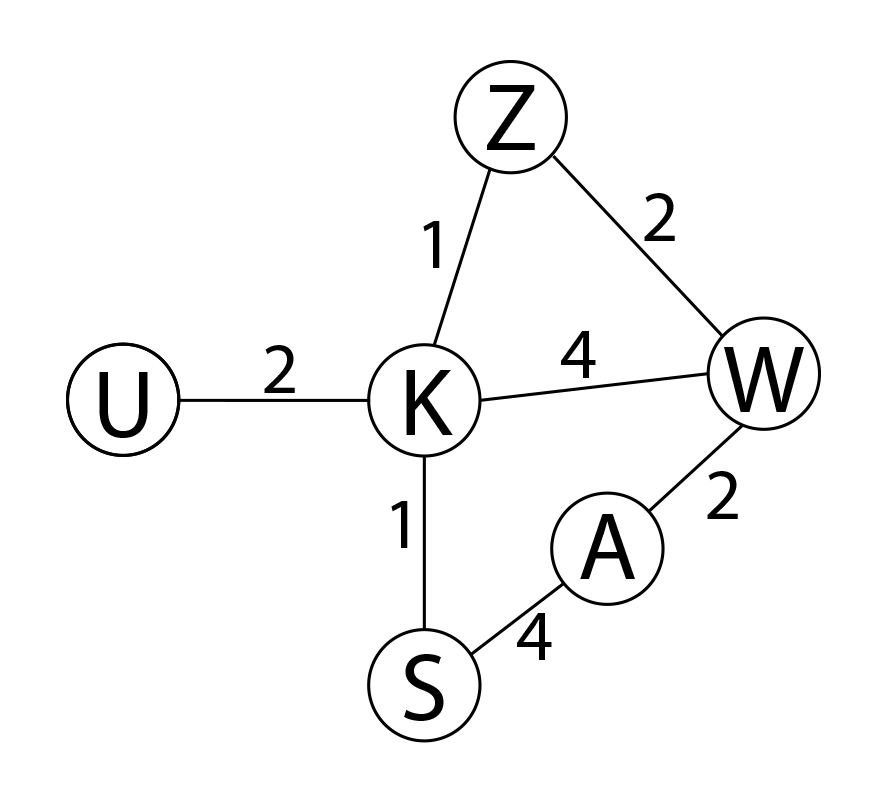
\includegraphics[width=8cm]{graph.png} 
   \caption{Graph des U-Bahn-Netz-Ausschnittes}
   \label{fig:example}
\end{figure}



\begin{table}[h]
   \centering
   %\topcaption{Table captions are better up top} % requires the topcapt package
   \begin{tabular}{@{} ccccccc @{}} % Column formatting, @{} suppresses leading/trailing space
      \toprule
      	Knoten & A & K &U & W & S & Z \\
      \midrule
      	A  & x & x & x & 2 & 4 & x \\
	K & x & x & 2 & 4  & 1 & 1 \\
	U  & x &  2 &x &  x &  x& x \\
	W  &  2 & 4 &x &x &x  &  2\\
	S  & 4 & 1 &x & x &  x& x \\
	Z  &  x& 1 & x& 2 & x & x \\

      \bottomrule
   \end{tabular}
   \caption{Adjazenzmatrix der U-Bahn-Verbindungen}
   \label{tab:booktabs}
\end{table}


\section*{Aufgabe 3.2 - Kürzester Weg mit Dijkstra}

\subsection*{Darstellung mit Priority Queue}

\begin{table}[h]
   \centering
   \begin{tabular}{@{} lcr @{}} % Column formatting, @{} suppresses leading/trailing space
      \toprule
      Schritt    & akt. Knoten & Priority-Queue \\
      \midrule
      0   	& - 			& U(-, 0) \\
       1        & U(-, 0)  		&  K(U, 2) \\
      2       	& K(U, 2)  		& S(K, 3), Z(K, 3), W(K, 6) \\
      3       	& S(K, 3)  		& Z(K, 3), W(K, 6)\\
      4 	& Z(K, 3)   	&  W(Z, 5), A(S, 7) \\
      5   	& W(Z, 5) 		&  A(W, 7), A(S, 7) \\
      6     	&  A(W, 7)	 	&  A(S, 7) \\
        \bottomrule
   \end{tabular}
   \caption{Darstellung des Dijkstra-Algorithmus mit Priority Queue }
   \label{tab:booktabs}
\end{table}
Anmerkung zu Schritt 4: Da mit W(Z, 5) ein definitiv kürzerer Weg besteht als W(K, 6), d.h. einer mit einem geringeren Gewicht, kann W(K, 6) verworfen werden.

Da in Schritt 5 A(W, 7) und A(S,7) das gleiche Gewicht haben, hängt es von der Implementierung der Priority Queue ab, welches Element im letzten Schritt als aktueller Knoten gewählt wird. Das bedeutet, dass es zwei gleichwertige Lösungen gibt nämlich: \\
\begin{itemize}
\item U - K - Z - W - A 
\item U - K - S - A
\end{itemize}

\subsection*{Darstellung in tabellarischer Form }


\begin{table}[h]
   \centering
   \begin{tabular}{@{} |c | c | c | c | c | c | c |@{}} % Column formatting, @{} suppresses leading/trailing space
      \toprule
      Schritt    & A & K & S & U & W & Z\\
      \midrule
      0 & - & - & - & 0 & - & - \\
      1 & - & U, 2 & - & 0 & - & - \\
      2 & - & U, 2 & K, 3 & 0 & K, 6 & K, 3 \\
      3 & S, 7 & U, 2 & K, 3 & 0 & Z, 5 & K, 3 \\
      4 & S, 7 & U, 2 & K, 3 & 0 & Z, 5 & K, 3 \\
      \bottomrule
   \end{tabular}
   \caption{Tabellarische Darstellung des Dijkstra-Algorithmus}
   \label{tab:booktabs}
\end{table}

Auch wenn sich im vierten Schritt gegenüber dem vorletzten nichts verändert, wird er durchgeführt, weil in Schritt 3 das Gesamtgewicht des Pfades bis Knoten W noch geringer ist als (S, 7). Deswegen wird im letzten Schritt noch von W aus weitergesucht. Je nach Implementierung könnte auch hier der alternative Pfad als Ergebnis herauskommen. Dann würde in der Spalte A (W, 7) in Zeile 4 stehen.

\end{document}